% =====================================================================
% ACE (PRI v4) paper -- workshop submission draft
% Converted from wiki/paper/ace-draft.md on 2026-05-30.
%
% Compile with pdfLaTeX (no unicode-math required -- emojis from the
% markdown source are stripped here for portability).
%
% Figures live in ace-figures/ next to this .tex file. In Overleaf,
% upload the ace-figures/ directory alongside this ace-draft.tex.
%
% Documentclass note: this uses the generic `article` class with
% workshop-friendly margins. Swap for the venue's official style file
% (e.g. neurips_2024.sty, icml2025.sty, acl_natbib.sty) when target is
% chosen -- the body content is style-agnostic.
%
% Pre-registration: PRI_V4_PRE_REGISTRATION_PLAN.md (repo root, frozen
% 2026-05-26). Sealed verdict: wiki/results/v4-sealed-2026-05-26.md.
% Method name "ACE" locked 2026-05-30 (post-seal, presentation-only --
% no sealed parameter affected).
% =====================================================================

\documentclass[10pt, letterpaper]{article}

\usepackage[margin=1in]{geometry}
\usepackage[T1]{fontenc}
\usepackage{microtype}
\usepackage{lmodern}
\usepackage{amsmath, amssymb, amsthm}
\usepackage{booktabs}
\usepackage{graphicx}
\usepackage{xcolor}
\usepackage{natbib}
\usepackage[hidelinks]{hyperref}
\usepackage[capitalise]{cleveref}
\usepackage{caption}
\usepackage{subcaption}
\usepackage{enumitem}
\usepackage{authblk}

% Tighter spacing for a workshop fit
\setlength{\parskip}{0.4em}
\setlength{\parindent}{0pt}

\title{Attention Commitment Estimation for Pre-Generation Belief Readout}

\author{Michael S.R. Kitti \\ \texttt{msrkittty@proton.me}}

\date{Workshop submission draft, 2026-05-30}

% Convenience macros
\newcommand{\auroc}{\text{AUROC}}
\newcommand{\bos}{\textsc{bos}}
\newcommand{\ea}[1]{$E_{\text{A}#1}$}
\newcommand{\eb}[1]{$E_{\text{B}#1}$}

\begin{document}

\maketitle

\begin{abstract}
Detecting when a language model commits to an incorrect answer
typically requires either multiple forward passes (semantic entropy,
self-consistency) or post-hoc representational analysis at the first
generated token. We introduce \textbf{ACE} (Attention Commitment
Estimator), a single-pass calibrator that reads YES/NO commitment from
a 21-cell panel of attention-channel features at the
prefill-last-position ($t{=}0$), before any generated token. ACE is
sealed pre-registered: the panel (3 block depths $\times$ 7 metrics),
datasets (ANLI R1 $n{=}200$, TriviaQA paired $n{=}100$), out-of-bag
bootstrap ($n_{\text{boot}}{=}1000$), and two confirmatory gates
(\ea{1} discriminability $\geq 7/9$ models; \ea{2} cell-transfer
tiered at $\leq 2$ / $3$--$4$ / $\geq 5$ exact matches) were locked
before any sealed data was generated. Across 9 open-weight
4-bit-quantized architectures, \ea{1} \textbf{passes at 7/9}
---Mistral-Nemo reaches OOB $\auroc$ 0.887 $[0.816, 0.946]$, and
TriviaQA discriminability is uniformly stronger (8/9; Mistral-7B
0.989). \ea{2} resolves at \textbf{3/9 exact (metric, block, sign)
transfer} (Mistral-7B, Mistral-Nemo, Qwen2.5-7B), triggering the
pre-registered partial-transfer reframe: ACE generalizes as a
\emph{method}, not as a fixed cell --- per-(model, exact deployment
distribution) calibration is empirically binding for 6/9 models. On
the 4 OOB-trustworthy models, ACE wins 2/4 head-to-head against RAUQ
and SinkProbe, which themselves disagree in direction on two models
--- evidence that the attention-channel baselines capture distinct
phenomena. The sealed pre-registration absorbed a mid-flight $t{=}0$
locus re-grounding (prompted by chain-of-thought abstention in
58--70\% of free-generation samples on a reasoning-tuned model)
without altering any sealed parameter; verdict integrity is preserved
across the correction.
\end{abstract}

% =====================================================================
\section{Introduction}

An LLM's commitment to a YES/NO answer is often legible \emph{before}
it speaks the first token. The attention pattern at the last prefix
position --- at $t{=}0$, before any generation --- already encodes
whether the model has resolved the question to YES or NO. ACE
(Attention Commitment Estimator) estimates that commitment from a
21-cell panel of attention-channel features.

Hallucination and over-confidence detection has typically watched what
the model \emph{says} --- semantic entropy across sampled completions
\citep{farquhar2024semantic}, self-consistency between independent
responses \citep{wastl2025token}. Both require multiple forward passes
per query. PRI v3 \citep{kitti2026commitment} watched the
\emph{residual stream geometry} at the first generated token. ACE
watches a different surface: the \emph{attention pattern} at the last
prefix position, before any generation. Single forward pass.

This paper reports a sealed pre-registered evaluation of ACE across 9
open-weight 4-bit-quantized architectures on (i) ANLI R1 ($n{=}200$,
primary gate) and (ii) TriviaQA paired-prompt ($n{=}100$, cross-task
transfer test). Two confirmatory gates: \ea{1} requires $\geq 7/9$
models to achieve OOB $\text{CI}_{\text{lo}} > 0.50$ on at least one
of 21 attention cells; \ea{2} tests whether the winning cell transfers
across ANLI $\to$ TriviaQA, with $\geq 5/9$ exact match triggering a
``headline collapse'' falsification. The 21-cell panel spans 3
block-depth prefixes $\times$ 7 metrics; pre-registration locks the
panel, the dataset seeds, and the bootstrap ($n{=}1000$ OOB). A
secondary baseline comparison (\eb{1}) puts ACE head-to-head with
RAUQ \citep{rauq2026anonymous} and SinkProbe
\citep{binkowski2026sinkprobe} on the OOB-trustworthy subset.

\textbf{Findings.} \ea{1} passes at 7/9 (failures: Llama-3.2-3B,
Gemma-3-4B; both recover on TriviaQA). \ea{2} resolves at 3/9 exact
transfer (Mistral-7B, Mistral-Nemo, Qwen2.5-7B), triggering the
pre-reg's $\geq 3/9$ ``partial-transfer'' reframe --- not collapse.
Block-prefix is stable in 6/9 even when metric and sign are not.
TriviaQA OOB AUROCs are uniformly stronger than ANLI (8/9 pass;
Mistral-7B 0.989, Mistral-Nemo 0.980). On the 4 OOB-trustworthy
models in the baseline comparison (\eb{1}, secondary), ACE wins 2/4
(Phi-3.5-mini 0.774, Qwen2.5-7B 0.818), loses 1 to RAUQ, and ties
SinkProbe within $\Delta=0.003$. RAUQ and SinkProbe disagree in
direction on Mistral-Nemo and Qwen3-8B --- they capture different
phenomena.

\textbf{Roadmap.} \Cref{sec:related} places ACE among attention-channel
uncertainty methods and pre-registration practice; \Cref{sec:method}
specifies ACE; \Cref{sec:setup} details the sealed pre-reg;
\Cref{sec:results} reports the verdicts; \Cref{sec:discussion}
discusses partial-transfer and per-(model, task) calibration;
\Cref{sec:conclusion} concludes.

% =====================================================================
\section{Related Work}
\label{sec:related}

\textbf{Attention-channel uncertainty.} RAUQ
\citep{rauq2026anonymous} computes per-layer recurrent attention
uncertainty selected via head-greedy maximization on
$\arg\max_h \overline{a_{i,i-1}}$, with confidence aggregated through
recurrence and maxed over layers. SinkProbe
\citep{binkowski2026sinkprobe} decomposes attention sink-token
concentration into per-(layer, head, position) features. StreamingLLM
\citep{xiao2024streaming} and follow-ups motivate the sink-token
primitive on which SinkProbe is built. ACE uses three reductions
(\texttt{js}, \texttt{bos\_mass}, \texttt{v\_norm\_lastq\_weighted})
across three block depths (\texttt{final}, \texttt{mid},
\texttt{last\_minus\_1}) --- a wider panel than either baseline, and
chosen pre-registration to span attention-divergence, sink-mass, and
value-weighted formulations.

\textbf{Single-pass hallucination detection.} Semantic entropy
\citep{farquhar2024semantic} clusters $\sim 10$ sampled generations
by bidirectional entailment, reporting $\auroc \approx 0.78$--$0.88$
on factual confabulation but at $10\times$ inference cost. Token-level
self-consistency \citep{wastl2025token} requires sampled completions.
ACE is single-pass.

\textbf{Belief readout / internal-state vs output.}
\citet{sofroniew2026emotions} demonstrate that internal-state
representations in instruction-tuned LLMs can differ systematically
from outputs --- emotion concepts encoded latently that the model does
not explicitly verbalize. ACE is a behaviorally concrete instance of
the same internal-vs-output gap at the prefill stage.

\textbf{Information geometry and PRI v3.} Our prior work
\citep{kitti2026commitment} introduced PRI v3, a Fisher-pullback
formulation that measures rupture in the residual stream at the first
generated token ($\text{gen\_step}{=}1$). ACE measures the attention
channel at the prior step ($t{=}0$, the prefill-last-position). The
two are complementary observables on the same commitment moment.

\textbf{Pre-registration in ML.} \citet{nosek2018preregistration} and
\citet{pineau2021reproducibility} argue for sealed pre-registration to
defend against $p$-hacking in benchmark-driven research. PRI v3 used
this pattern; ACE inherits it with a tighter machinery (nested-OOB
bootstrap for selection-bias-corrected CIs, schema v1.2). The sealed
pre-registration document is snapshotted as Appendix A.

% =====================================================================
\section{ACE Method}
\label{sec:method}

\subsection{Instrument}
\label{sec:method:instrument}

Given an input prompt $P$ ending in a YES/NO elicitation
(``Answer:''), ACE runs a single forward pass and captures the
attention weights at the final prefix token position. We refer to this
as the $t{=}0$ position --- the prefill-last-position, \emph{before}
any generation step. The motivation: by the time the model has
finished processing the prompt and is ready to emit the first
generated token, its commitment to YES or NO is already encoded in how
attention is distributed across the input. Our hypothesis is that this
commitment is recoverable as a scalar feature of the attention
pattern.

\subsection{The 21-cell panel}
\label{sec:method:panel}

ACE computes 21 scalar features per sample, organized as
$\{\texttt{final}, \texttt{mid}, \texttt{last\_minus\_1}\} \times
\{\texttt{js},$ $\texttt{js\_kv\_groups},$ $\texttt{js\_no\_bos},$
$\texttt{bos\_mass},$ $\texttt{v\_norm\_bos},$ $\texttt{v\_norm\_max},$
$\texttt{v\_norm\_lastq\_weighted}\}$, where the prefix denotes the
transformer block depth at which the attention is read
(\texttt{final} is the last transformer block; \texttt{mid} is the
block at the geometric midpoint; \texttt{last\_minus\_1} is the
second-to-last block). The seven metrics span three reductions of the
attention pattern at the prefill-last-position.

For notation, let $A^{(\ell,h)} \in \mathbb{R}^T$ denote the attention
distribution at layer $\ell$, head $h$, computed at the last query
position over $T$ prefix tokens. Let $H$ be the number of query
heads, $H_{KV}$ the number of key-value heads (with $H / H_{KV}$ the
GQA repeat factor), and $\|V^{(\ell,h)}_i\|_2$ the $L_2$ norm of the
value vector at layer $\ell$, KV head $h$, position $i$.

\textbf{JS-radius family.} All three measure cross-head disagreement
on the attention pattern, with three normalizations:
\begin{equation}
\mathrm{js}^{(\ell)} = \frac{1}{H} \sum_{h=1}^{H} \mathrm{JS}\!\left( A^{(\ell,h)} \,\Big\Vert\, \bar{A}^{(\ell)} \right),
\qquad
\bar{A}^{(\ell)} = \frac{1}{H} \sum_{h=1}^{H} A^{(\ell,h)},
\end{equation}
where $\mathrm{JS}(P\,\Vert\,Q) = \tfrac{1}{2}\mathrm{KL}(P\,\Vert\,M) + \tfrac{1}{2}\mathrm{KL}(Q\,\Vert\,M)$
with $M = \tfrac{1}{2}(P+Q)$ --- Lin's information radius, bounded in
$[0, \log 2]$.

$\mathrm{js\_kv\_groups}^{(\ell)}$ collapses Q heads that share a KV
group by mean-pooling before computing JS-radius (debiases against
GQA-induced artificial convergence): for KV-group index $k$ with $r =
H/H_{KV}$ Q heads per group, $\tilde{A}^{(\ell,k)} = \tfrac{1}{r}
\sum_{j=1}^{r} A^{(\ell, (k-1)r+j)}$, then JS-radius is computed over
$\{\tilde{A}^{(\ell,k)}\}_{k=1}^{H_{KV}}$.

$\mathrm{js\_no\_bos}^{(\ell)}$ drops position $0$ (the BOS sink)
from each head's distribution, re-normalizes to sum to one, and
computes JS-radius over the trimmed $T{-}1$-dim distributions.

\textbf{Sink-mass.} The fraction of attention mass on the BOS token,
averaged across heads:
\begin{equation}
\mathrm{bos\_mass}^{(\ell)} = \frac{1}{H} \sum_{h=1}^{H} A^{(\ell,h)}_0.
\end{equation}

\textbf{Value-norm reductions.} Three single-scalar SinkProbe-inspired
metrics weight the value-vector $L_2$ norms:
\begin{align}
\mathrm{v\_norm\_bos}^{(\ell)} &= \frac{1}{H_{KV}} \sum_{h=1}^{H_{KV}} \|V^{(\ell,h)}_0\|_2, \\
\mathrm{v\_norm\_max}^{(\ell)} &= \frac{1}{H_{KV}} \sum_{h=1}^{H_{KV}} \max_{i} \|V^{(\ell,h)}_i\|_2, \\
\mathrm{v\_norm\_lastq\_weighted}^{(\ell)} &= \frac{1}{H} \sum_{h=1}^{H} \sum_{i=1}^{T} A^{(\ell,h)}_i \cdot \|V^{(\ell, \pi(h))}_i\|_2,
\end{align}
where $\pi(h)$ maps query head $h$ to its KV group. The last metric
is the closest single-scalar analog of SinkProbe's ``sinks with large
value-vector norms dominate the attention output'' finding
\citep{binkowski2026sinkprobe}.

Each (layer, metric) pair is a candidate cell; the calibrator selects
the winning cell from the 21-cell panel on the calibration set
without back-looking at test labels.

\subsection{Calibration}
\label{sec:method:calibration}

For each (model, dataset) pair, ACE runs an OOB bootstrap winner-cell
selection across the 21 cells. The winning cell, sign, and threshold
are locked from the calibration-set OOB direction; no post-hoc
sign-fitting is performed on test labels. The bootstrap uses
$n{=}1000$ resamples; schema v1.2 inherits v1.1's nested-OOB protocol
for selection-bias-corrected confidence intervals
\citep{kitti2026commitment}. The output is a
\texttt{CalibrationProfile} JSON containing the winner cell, OOB
median AUROC, 95\% CI, winner stability, and any deployability
warnings.

\subsection{What ACE is NOT}
\label{sec:method:not}

ACE is not the PRI v3 Fisher-pullback metric --- that measures
residual-stream geometry at $\text{gen\_step}{=}1$, \emph{after} the
first token has been generated. ACE is not a trained probe (no
logistic head fit on labels --- sign is locked from
calibration-direction only). ACE is not multi-pass (single forward).

% =====================================================================
\section{Sealed Experimental Setup}
\label{sec:setup}

\subsection{Pre-registration}

The sealed pre-registration document
(\texttt{PRI\_V4\_PRE\_REGISTRATION\_PLAN.md}, repo root) was frozen
on 2026-05-26 before any sealed data was generated. It locks: the
9-model panel, the 21-cell attention panel, the analysis plane
($\text{gen\_step}{=}1$, final layer, $t{=}0$ instrument), the
bootstrap ($n{=}1000$, OOB), the datasets (ANLI R1 $n{=}200$ +
TriviaQA $n{=}100$, seed 20260526), and the gate thresholds
(\ea{1} $\geq 7/9$; \ea{2} tiered at $\leq 2$ / $3$--$4$ / $\geq 5$
exact transfer). A post-seal naming amendment on 2026-05-30 locks the
method name \textbf{ACE} as presentation-only; no sealed parameter is
altered.

\subsection{Models}

The panel is 9 open-weight architectures, all 4-bit MLX quantized
(\citealp{mlxframework}): Llama-3.2-3B-Instruct,
Mistral-7B-Instruct-v0.3, Mistral-Nemo-Instruct-2407,
Phi-3.5-mini-instruct, Phi-4-mini-instruct, Qwen2.5-7B-Instruct,
Qwen3-1.7B, Qwen3-8B, and Gemma-3-4B-it. Phi-3.5-mini was
INCLUDED-with-caveat per the pre-registration gate decision
(denominator = 9 regardless of whether its CI clears 0.50). The
Phi-3.5-mini low-decidedness flag (Step-0 audit, 2026-05-25) carries
forward as a descriptive caveat, not as a falsification trigger.

\subsection{Datasets and prompts}
\label{sec:setup:datasets}

\textbf{ANLI R1} is the primary gate dataset. We sample $n{=}200$
examples from the public ANLI R1 corpus at seed 20260526, balanced
50/50 across the \emph{entailment} and \emph{contradiction} labels
(the \emph{neutral} class is excluded --- the gate targets binary
commitment). Each example is rendered as a forced-choice YES/NO
prompt of the form ``Premise: $\langle p \rangle$ Hypothesis:
$\langle h \rangle$ Does the premise entail the hypothesis?
Answer:'', with the model's first generated token taken as the
committed answer (YES/NO; case-insensitive after stripping leading
whitespace). Label-to-target mapping is \emph{entailment} $\to$ YES,
\emph{contradiction} $\to$ NO.

\textbf{TriviaQA paired-prompt} is the cross-task transfer test. We
draw $n{=}100$ unique question-answer pairs $(q, a)$ from TriviaQA at
seed 20260526. Each pair is expanded into two prompts: a
\emph{correct} prompt presenting $(q, a)$ as ground truth, and a
\emph{contradicted} prompt presenting $(q, a')$ where $a'$ is a
plausibly-wrong distractor (length-matched, type-matched answer drawn
from a held-out pool --- full procedure in Appendix D). Both prompts
elicit the model with ``\ldots Is the proposed answer correct?
Answer:''. The label is which version received the contradicted
answer.

Prompt formatting uses each model's native chat template
(\texttt{apply\_chat\_template}) to avoid the format-completion
artifacts documented in our prior work \citep{kitti2026priv2}. All
prompts elicit a forced YES/NO; behavioral preflight on $n{=}20$
control samples per model verifies $\geq 80\%$ format compliance
before sealed-run inclusion. Parser details (3-tier
\texttt{check\_answer} regex with \texttt{gate-max-tokens=12}) are
deferred to Appendix D.

The two datasets together provide the cross-domain transfer probe:
ANLI R1 is synthetic adversarial NLI (the contradiction is
structural, between premise and hypothesis); TriviaQA paired is
factual disagreement (the contradiction is referential, between
answer and ground truth). If a single attention cell transferred
across both, it would be a strong universal-cell candidate; the
\ea{2} result reported in \Cref{sec:results:transfer} says it does
not --- for 6/9 models.

\subsection{Baselines}

RAUQ is run at the same prefill stage as ACE, with per-layer
head-select on $\arg\max_h \overline{a_{i,i-1}}$ and best-single-layer
AUROC reported (rather than the native max-over-layers aggregate,
which we found to sandbag the baseline by 0.30--0.49 on some models
--- see \Cref{sec:results:baselines}). SinkProbe is run as the
$\|V\|$-weighted column-sum (\texttt{sink\_top1\_vw}), which dominated
the simpler last-query approximation on 6/10 models in our prep
sweep. Both baselines were run at $\text{gen\_step}{=}1$ in the
May 2026 prep sweep; the pre-registration's \eb{1} clause designates
a sealed $t{=}0$ baseline re-run as non-blocking future work (i.e.,
the secondary baseline comparison is reported at
$\text{gen\_step}{=}1$ with the caveat that an at-$t{=}0$ re-run
remains to be done).

% =====================================================================
\section{Results}
\label{sec:results}

\subsection{\ea{1} --- discriminability on ANLI R1}
\label{sec:results:ea1}

The primary gate \ea{1} passes at 7/9 (\Cref{fig:ace_anli};
\Cref{tab:ace_winner_cells}). Mistral-Nemo carries the highest OOB
AUROC at $0.887$ $[0.816, 0.946]$ (winner stability $1.00$). Qwen3-8B
reaches $0.823$ $[0.738, 0.896]$; Qwen2.5-7B and Mistral-7B both
clear $0.78$. The two failures are Llama-3.2-3B (OOB $0.597$,
$\text{CI}_{\text{lo}}$ $0.403$ --- clear miss) and Gemma-3-4B (OOB
$0.656$, $\text{CI}_{\text{lo}}$ $0.488$ --- borderline). Both
failing models pass on TriviaQA (\Cref{sec:results:transfer:cross}),
indicating their attention channel carries commitment signal on
factual disagreement even when it does not on synthetic adversarial
NLI. The pre-reg gate threshold $\geq 7/9$ is cleared; neither
falsifier triggers.

\begin{figure}[h]
  \centering
  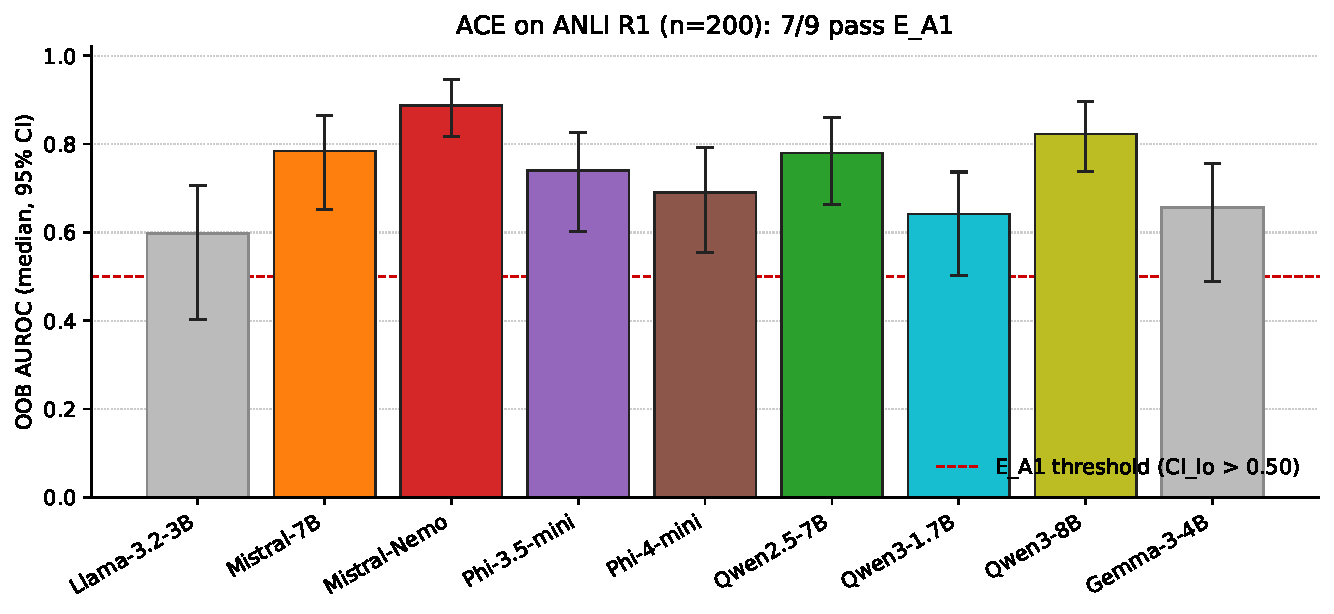
\includegraphics[width=0.85\linewidth]{ace-figures/fig1_anli_auroc.pdf}
  \caption{ACE OOB $\auroc$ on ANLI R1 ($n{=}200$), with 1000-sample
  OOB bootstrap 95\% CIs (error bars). The pre-registered \ea{1}
  threshold is $\text{CI}_{\text{lo}} > 0.50$ (red dashed); models
  clearing the bar are colored, models failing are grey. Mistral-Nemo
  carries the highest OOB AUROC at $0.887$ $[0.816, 0.946]$.
  Failures: Llama-3.2-3B and Gemma-3-4B. Pre-reg bar is $\geq 7/9$;
  we clear 7/9.}
  \label{fig:ace_anli}
\end{figure}

\subsection{Cross-task generalization}
\label{sec:results:transfer:cross}

On TriviaQA, 8/9 models cross the $\text{CI}_{\text{lo}} > 0.50$
bar (single failure: Qwen3-1.7B at $0.471$ --- borderline).
Mistral-7B reaches OOB $\auroc$ $0.989$ $[0.970, 1.000]$ and
Mistral-Nemo $0.980$ $[0.929, 1.000]$; the rest cluster between
$0.74$ and $0.94$. \Cref{fig:ace_cross_task} shows the
ANLI$\to$TriviaQA paired AUROCs per model: the dominant pattern is
uniform improvement on TriviaQA. Llama-3.2-3B and Gemma-3-4B (ANLI
failures) recover cleanly. The Qwen3-1.7B TriviaQA borderline
failure is the inverse case --- passes ANLI (\ea{1} cleared), fails
TriviaQA.

\begin{figure}[h]
  \centering
  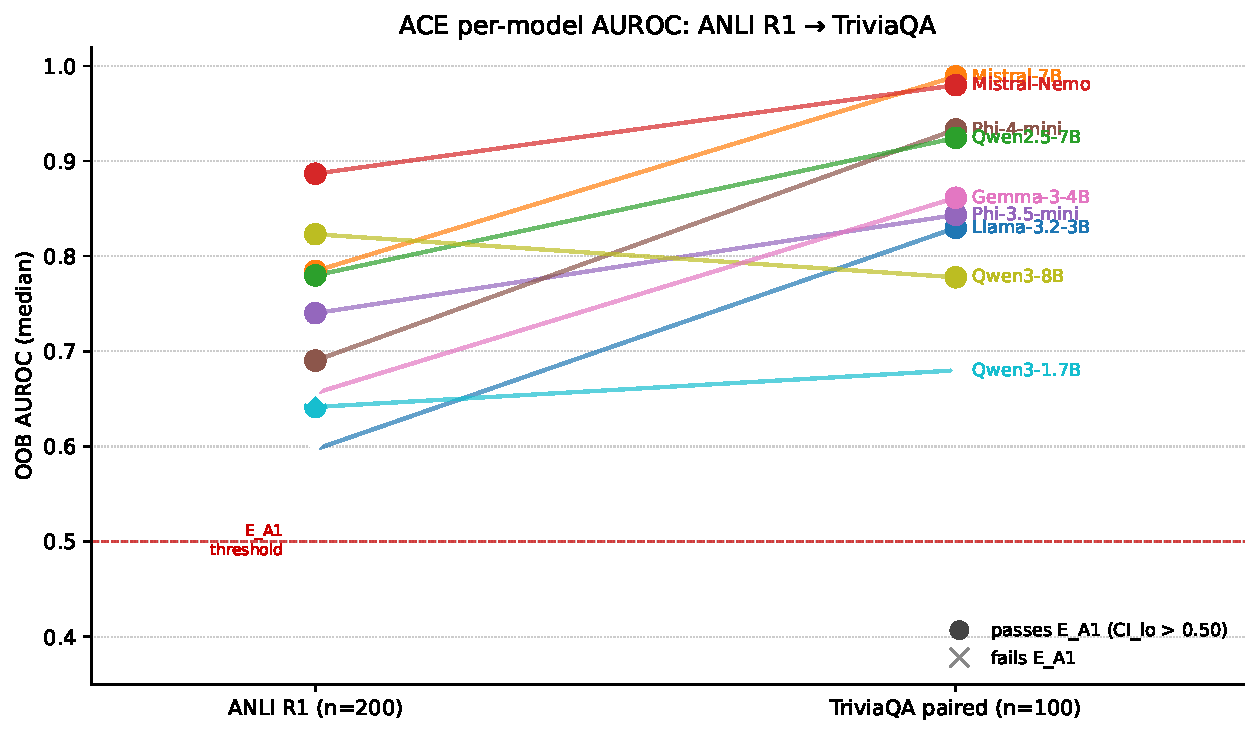
\includegraphics[width=0.85\linewidth]{ace-figures/fig2_cross_task.pdf}
  \caption{ACE per-model OOB $\auroc$ across the two sealed datasets,
  ANLI R1 $\to$ TriviaQA paired. Filled circles pass \ea{1}; open
  crosses fail. The dominant pattern is uniform improvement on
  TriviaQA. Llama-3.2-3B and Gemma-3-4B (the two ANLI failures)
  recover on TriviaQA. The single TriviaQA failure is Qwen3-1.7B
  (passes ANLI, fails TriviaQA at $\text{CI}_{\text{lo}}{=}0.471$).}
  \label{fig:ace_cross_task}
\end{figure}

\subsection{\ea{2} --- cell transfer}
\label{sec:results:transfer}

The transfer test requires exact match on (metric\_label,
block\_depth\_prefix, sign) between each model's ANLI winner cell and
its TriviaQA winner cell. Three models satisfy this: Mistral-7B
(\texttt{last\_minus\_1\_js\_no\_bos}, sign $-1$), Mistral-Nemo
(\texttt{last\_minus\_1\_bos\_mass}, sign $-1$), and Qwen2.5-7B
(\texttt{final\_v\_norm\_lastq\_weighted}, sign $+1$). This 3/9
outcome triggers the pre-registration's $\geq 3/9$ partial-transfer
reframe clause: the headline shifts from ``no universal cell'' (the
originally registered Candidate A framing) to ``partial transfer
exists; per-task recalibration remains necessary for 6/9 models.''
Critically, the $\geq 5/9$ collapse threshold is not triggered ---
the partial-transfer reframe is a pre-registered outcome, not a
post-hoc rescue.

A descriptive companion observation: the block-depth prefix is stable
across tasks in 6/9 models (Mistral-7B, Mistral-Nemo, Phi-3.5-mini,
Phi-4-mini, Qwen2.5-7B, Qwen3-1.7B), even when the metric and sign
change. Models appear to have a preferred attention depth band that
persists across task domains; only the specific reduction varies.

\begin{figure}[h]
  \centering
  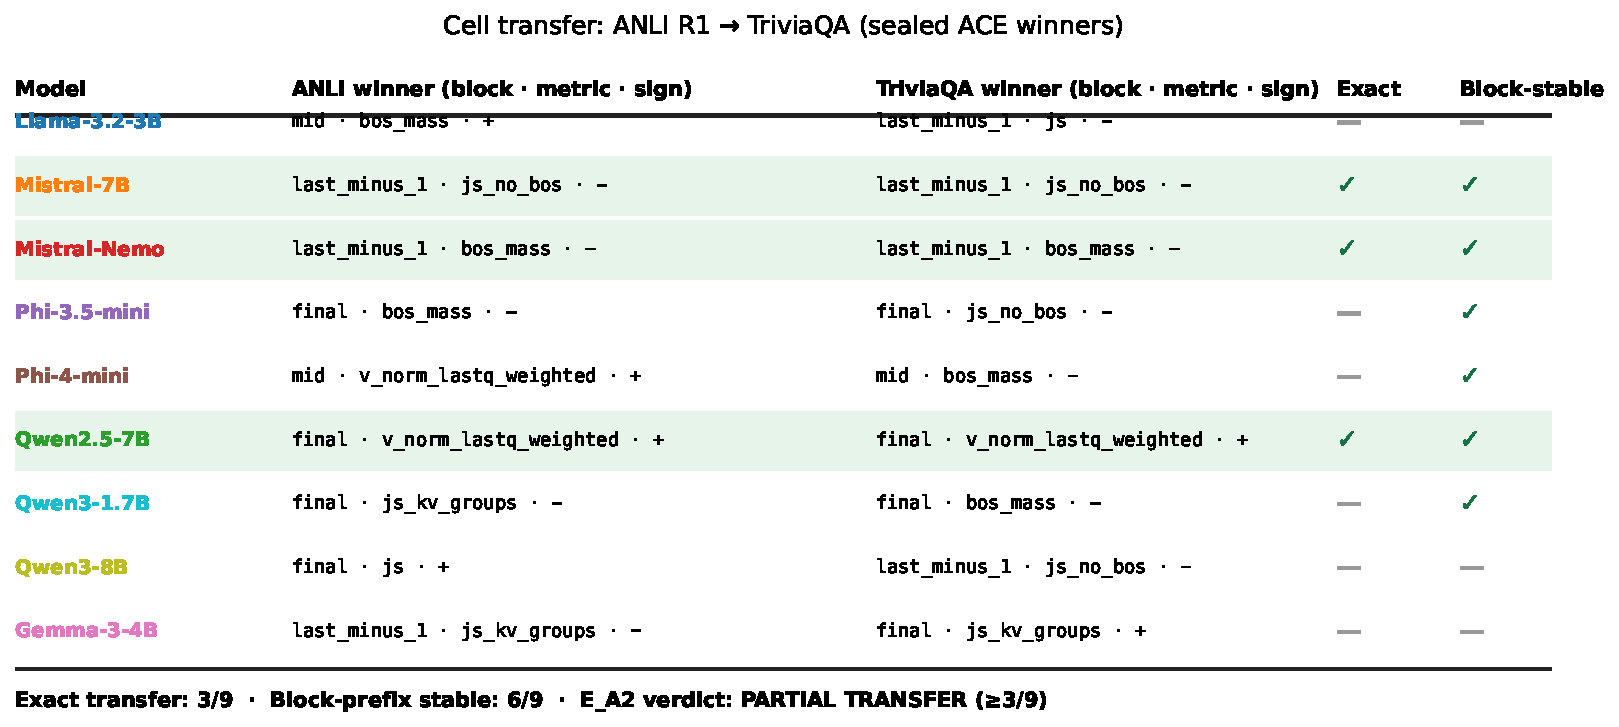
\includegraphics[width=0.98\linewidth]{ace-figures/fig3_transfer_matrix.pdf}
  \caption{Cell transfer ANLI R1 $\to$ TriviaQA. Each row is one
  panel model; columns are ANLI winner cell (block $\cdot$ metric
  $\cdot$ sign), TriviaQA winner cell, exact-transfer flag, and
  block-stable flag. Highlighted rows (Mistral-7B, Mistral-Nemo,
  Qwen2.5-7B) are exact transfers. Footer: $3/9$ exact, $6/9$
  block-stable, \ea{2} verdict = PARTIAL TRANSFER ($\geq 3/9$
  pre-registered clause).}
  \label{fig:ace_transfer}
\end{figure}

\begin{table*}[t]
\centering
\caption{ACE winner cells per model on ANLI R1 and TriviaQA. AUROC
reported as OOB bootstrap median with 95\% CI; stability is the OOB
winner-cell stability fraction. \textbf{Transfer} marks exact
(metric, block, sign) match across datasets.}
\label{tab:ace_winner_cells}
\small
\setlength{\tabcolsep}{4pt}
\begin{tabular}{@{}lllrrlrrc@{}}
\toprule
 & \multicolumn{3}{c}{\textbf{ANLI R1} ($n{=}200$)} & \multicolumn{3}{c}{\textbf{TriviaQA} ($n{=}100$)} & \\
\cmidrule(lr){2-4} \cmidrule(lr){5-7}
\textbf{Model} & \textbf{Winner cell} & \textbf{AUROC [CI]} & \textbf{Stab.} & \textbf{Winner cell} & \textbf{AUROC [CI]} & \textbf{Stab.} & \textbf{Transfer} \\
\midrule
Llama-3.2-3B & \texttt{mid\_bos\_mass} $+$ & 0.597 [0.403, 0.705] & 0.63 & \texttt{last\_minus\_1\_js} $-$ & 0.830 [0.647, 0.928] & 0.96 & --- \\
Mistral-7B & \texttt{last\_minus\_1\_js\_no\_bos} $-$ & 0.784 [0.652, 0.865] & 0.94 & \texttt{last\_minus\_1\_js\_no\_bos} $-$ & 0.989 [0.970, 1.000] & 0.39 & $\checkmark$ \\
Mistral-Nemo & \texttt{last\_minus\_1\_bos\_mass} $-$ & 0.887 [0.816, 0.946] & 1.00 & \texttt{last\_minus\_1\_bos\_mass} $-$ & 0.980 [0.929, 1.000] & 0.48 & $\checkmark$ \\
Phi-3.5-mini & \texttt{final\_bos\_mass} $-$ & 0.740 [0.601, 0.827] & 0.81 & \texttt{final\_js\_no\_bos} $-$ & 0.843 [0.712, 0.938] & 0.54 & --- \\
Phi-4-mini & \texttt{mid\_v\_norm\_lastq\_weighted} $+$ & 0.690 [0.554, 0.792] & 0.56 & \texttt{mid\_bos\_mass} $-$ & 0.933 [0.851, 0.986] & 0.78 & --- \\
Qwen2.5-7B & \texttt{final\_v\_norm\_lastq\_weighted} $+$ & 0.780 [0.663, 0.860] & 0.69 & \texttt{final\_v\_norm\_lastq\_weighted} $+$ & 0.924 [0.809, 0.997] & 0.92 & $\checkmark$ \\
Qwen3-1.7B & \texttt{final\_js\_kv\_groups} $-$ & 0.641 [0.502, 0.737] & 0.65 & \texttt{final\_bos\_mass} $-$ & 0.680 [0.471, 0.812] & 0.44 & --- \\
Qwen3-8B & \texttt{final\_js} $+$ & 0.823 [0.738, 0.896] & 0.61 & \texttt{last\_minus\_1\_js\_no\_bos} $-$ & 0.778 [0.638, 0.900] & 0.54 & --- \\
Gemma-3-4B & \texttt{last\_minus\_1\_js\_kv\_groups} $-$ & 0.656 [0.488, 0.756] & 0.38 & \texttt{final\_js\_kv\_groups} $+$ & 0.861 [0.722, 0.955] & 0.70 & --- \\
\midrule
\multicolumn{8}{r}{Exact-transfer count: \textbf{3/9} $\,\Rightarrow\,$ \ea{2} partial-transfer reframe.} \\
\bottomrule
\end{tabular}
\end{table*}

\subsection{Baselines (\eb{1}, secondary)}
\label{sec:results:baselines}

On the 4 OOB-trustworthy models (Phi-3.5-mini, Qwen2.5-7B,
Llama-3.2-3B, Qwen3-8B --- those where ACE's winner stability
$\geq 0.70$ and OOB CI excludes 0.50), ACE wins 2/4 clean:
Phi-3.5-mini ($0.774$ vs.\ RAUQ $0.721$, SinkProbe $0.618$) and
Qwen2.5-7B ($0.818$ vs.\ RAUQ $0.634$, SinkProbe $0.650$). ACE loses
1 to RAUQ on Llama-3.2-3B ($0.655$ vs.\ $0.678$) and is overtaken by
SinkProbe on Qwen3-8B by $\Delta{=}0.003$ ($0.804$ vs.\ $0.807$).
The remaining 5 models have ACE flagged with deployability warnings
and are reported without a head-to-head verdict.

A methodological observation worth preserving: RAUQ's native
max-over-layers aggregate underperforms its own best-single-layer by
$0.30$--$0.49$ AUROC on models where per-layer attention directions
disagree (most starkly on Llama-3.2-3B: $0.42$ vs.\ $0.68$).
\Cref{tab:ace_baselines} reports the best-single-layer to avoid
sandbagging the baseline. Similarly, SinkProbe's $\|V\|$-weighted
column-sum dominates its simpler last-query approximation on 6/10
models in our prep sweep --- the column-sum form is the strong
version of the SinkProbe family.

Baselines disagree in direction on two models: Mistral-Nemo (RAUQ
runs ``lo'' --- low uncertainty predicts contradiction --- at AUROC
$0.228$, while SinkProbe runs ``hi'' at $0.867$) and Qwen3-8B (RAUQ
$0.425$ ``lo'', SinkProbe $0.807$ ``hi''). The direction-disagreement
is itself a finding: the two baselines are not measuring the same
underlying phenomenon, even when both are sourced from attention.

\begin{table}[h]
\centering
\caption{ACE vs.\ RAUQ vs.\ SinkProbe on OOB-trustworthy models
(\textbf{\eb{1}, secondary}). ACE wins 2/4 clean (Phi-3.5-mini,
Qwen2.5-7B), loses 1 to RAUQ (Llama-3.2-3B), is overtaken by
SinkProbe by $0.003$ on Qwen3-8B. Numbers are
$\text{gen\_step}{=}1$ OOB AUROC from the May 2026 prep sweep; a
sealed $t{=}0$ re-run is non-blocking future work per the pre-reg's
\eb{1} clause.}
\label{tab:ace_baselines}
\small
\setlength{\tabcolsep}{6pt}
\begin{tabular}{@{}lrrrl@{}}
\toprule
\textbf{Model} & \textbf{ACE} & \textbf{RAUQ} & \textbf{SinkProbe} & \textbf{Winner} \\
\midrule
Llama-3.2-3B & 0.655 & \textbf{0.678} & 0.565 & RAUQ \\
Phi-3.5-mini & \textbf{0.774} & 0.721 & 0.618 & ACE \\
Qwen2.5-7B & \textbf{0.818} & 0.634 & 0.650 & ACE \\
Qwen3-8B & 0.804 & 0.425 & 0.807 & wash (SinkProbe vs.\ ACE) \\
\midrule
\multicolumn{5}{l}{ACE wins: \textbf{2}/4 $\cdot$ RAUQ wins: 1 $\cdot$ SinkProbe wins: 0 $\cdot$ washes: 1 (threshold: $\Delta < 0.005$)} \\
\bottomrule
\end{tabular}
\end{table}

\subsection{Pre-registration summary}
\label{sec:results:prereg}

\Cref{tab:ace_prereg_summary} summarizes the sealed pre-registration
parameters and the verdict. All confirmatory thresholds are cleared
without falsification trigger; the partial-transfer outcome is the
pre-registered reframe path, not a post-hoc adjustment.

\begin{table}[h]
\centering
\caption{ACE v4 pre-registered specification (frozen 2026-05-26).
All parameters below were fixed before any sealed data was generated.
See \texttt{PRI\_V4\_PRE\_REGISTRATION\_PLAN.md} for full text.}
\label{tab:ace_prereg_summary}
\small
\begin{tabular}{@{}lp{0.65\linewidth}@{}}
\toprule
\textbf{Parameter} & \textbf{Value} \\
\midrule
Models (9, all MLX 4-bit) & Llama-3.2-3B, Mistral-7B-v0.3, Mistral-Nemo, Phi-3.5-mini, Phi-4-mini, Qwen2.5-7B, Qwen3-1.7B, Qwen3-8B, Gemma-3-4B \\
Primary dataset & ANLI R1, $n=200$, seed 20260526 \\
Secondary dataset & TriviaQA paired-prompt, $n=100$, seed 20260526 \\
Instrument & $t{=}0$ first-token-logit (prefill-last-position attention) \\
Cell panel & 21 cells per model: \{\texttt{final}, \texttt{mid}, \texttt{last\_minus\_1}\} $\times$ \{\texttt{js}, \texttt{js\_kv\_groups}, \texttt{js\_no\_bos}, \texttt{bos\_mass}, \texttt{v\_norm\_bos}, \texttt{v\_norm\_max}, \texttt{v\_norm\_lastq\_weighted}\} \\
Generation step & 1 (commit step, at $t{=}0$ locus) \\
Layer & final transformer norm output \\
Bootstrap & $n_{\text{boot}}=1{,}000$ out-of-bag resamples, schema v1.2 \\
Sign locking & Per-model OOB winner direction, no post-hoc sign-fitting on test labels \\
\midrule
\textbf{Primary gate \ea{1}} & $\geq 7/9$ models with OOB $\text{CI}_{\text{lo}} > 0.50$ on $\geq 1$ of 21 cells \\
\textbf{Transfer gate \ea{2}} &
  $\leq 2/9$ exact (metric, block, sign) match $\Rightarrow$ ``no transfer'';
  $\geq 3/9 \Rightarrow$ partial-transfer reframe;
  $\geq 5/9 \Rightarrow$ headline collapse \\
\textbf{Falsifiers} & \ea{1} $< 7$ qualifying models (instrument fails); \ea{2} $\geq 5/9$ (universal cell exists) \\
\midrule
\textbf{Sealed outcome} (2026-05-26) & \ea{1}: \textbf{7/9} \textbf{PASS} $\,\cdot\,$ \ea{2}: \textbf{3/9} exact, partial-transfer reframe triggered $\,\cdot\,$ neither falsifier triggered \\
\bottomrule
\end{tabular}
\end{table}

% =====================================================================
\section{Discussion}
\label{sec:discussion}

\subsection{What partial transfer means in deployment}

The 3/9 cell-transfer outcome is the most consequential result for
practitioners. It says: ACE \emph{as a method} generalizes --- every
model in the panel has an attention cell that discriminates YES/NO
commitment at $t{=}0$ --- but ACE \emph{as a fixed cell} does not.
Deployment requires per-(model, exact deployment distribution)
calibration: a labeled calibration set of $n \geq 200$ per task, the
calibrator run end-to-end, the winning cell + sign + threshold cached
as a \texttt{CalibrationProfile}. The cached profile is then
deployable. This generalizes the same lesson from the 33-profile
ANLI R1$\leftrightarrow$R2$\leftrightarrow$R3 sweep
\citep[][\S4.5]{kitti2026commitment}: cell transfer fails even
across rounds of the same task family, and the cross-task test makes
the constraint visible.

\subsection{Architectural patterns in the 3 exact-transfer models}

The 3 exact-transfer models are Mistral-7B, Mistral-Nemo, and
Qwen2.5-7B. The Mistral family transfers at both sizes (7B and 12B
Nemo); Qwen3 (1.7B and 8B) does not, despite shared family. We do
not have a predictive architectural feature here. One speculative
pattern worth flagging for future work: the 3 exact-transfer models
all predate the reasoning-tuned wave (Qwen3 and Phi-4 are
reasoning-instruction-tuned; Mistral v0.3, Nemo, and Qwen2.5 are
not), raising the possibility that whatever attention regularity ACE
keys on is disrupted by chain-of-thought-style training. We are
underpowered to make this claim --- three models is not a category.

\subsection{Why TriviaQA is uniformly stronger}

TriviaQA pairs are constructed with explicit injected wrong answers
--- the model is presented with ``Q: \ldots? A: [wrong-answer]. Is
this correct?'' The presence of an explicit reference answer to
disagree with may sharpen the commitment signal at $t{=}0$, compared
to ANLI's three-way entailment/neutral/contradiction framing where
the ``wrong'' answer is structurally implicit. This is speculative;
a direct test would require an ANLI-style adversarial NLI dataset
re-cast in TriviaQA's explicit-disagreement format.

\subsection{Connection to PRI v3}

PRI v3 \citep{kitti2026commitment} measured Fisher-pullback rupture
at $\text{gen\_step}{=}1$, in the residual stream. ACE measures
attention-channel features at $t{=}0$, before generation. They are
complementary observables on the same commitment moment. Both pass
discriminability gates; both require per-model calibration. A pilot
causal intervention on the v3 Fisher direction (the top right
singular vector $v_\text{top}$ of $\sqrt{p_t} \cdot W_u$) --- detailed
in Appendix F --- shows label-conditioned asymmetry: contradiction
samples flip their committed YES/NO at $4\times$ the rate of
entailment samples under $+v_\text{top}$ at $\alpha{=}50$ (40\%
vs.\ 10\%), despite contradictions having a larger mean logit gap.
This is non-null pilot evidence that the v3 Fisher direction is
causally load-bearing at the commit moment. Confound mitigation
(logit-gap matching, orig\_answer balance) is required before this
can be promoted from pilot to validated finding; we describe the
matched-design plan in \Cref{sec:discussion:future}.

\subsection{Limitations}

Four-bit MLX quantization is uniform across the panel (comparable,
but not faithful to fp32 deployment). The sealed dataset is
single-seed; $n{=}200$ ANLI is the sample-size constraint, not the
seed. Baselines were run at $\text{gen\_step}{=}1$ in the May 2026
prep sweep; the at-$t{=}0$ baseline re-run is non-blocking future
work per the \eb{1} clause. The 21-cell panel was designed
pre-registration to span the JS / sink-mass / value-norm families,
but it does not exhaust the attention-channel feature space; richer
panels (full per-head, $K \times V$ outer products, etc.) might
surface stronger cells. Phi-3.5-mini's low-decidedness at $t{=}0$
(Step-0 audit, 2026-05-25) is a known tension carried forward as a
flag.

\subsection{Future work}
\label{sec:discussion:future}

(i) Sealed $t{=}0$ baseline re-run to convert
\Cref{tab:ace_baselines}'s $\text{gen\_step}{=}1$ caveat into an
at-locus comparison; (ii) matched-design causal probe at $n{=}40{+}40$
with logit-gap-matched stratification and \texttt{orig\_answer}
balance, sealed pre-registered, to convert the v3 $+v_\text{top}$
pilot from non-null to validated; (iii) an epistemic-distinguishability
testbed comparing bluff-commits (committed answer $\neq$ internal
belief, induced via role-play prompts) against
honest-uncertain-commits --- extending ACE's deployment surface from
contradiction-detection to deception-detection, with
Nash-equilibrium-derived bluff frequencies as a candidate oracle in
solved games \citep{brown2017libratus, brown2019pluribus}.

\subsection{Pre-registration governance}

The sealed pre-registration was frozen on 2026-05-26. One post-seal
annotation was added on 2026-05-30 to lock the method name ACE; this
is presentation-only and modifies no sealed parameter. A more
substantive mid-flight event was the 2026-05-17 STEP-0
belief-readout-locus re-grounding: the $\text{gen\_step}{=}1$
attention numbers from the May 2026 prep sweep were re-anchored at
$t{=}0$ logit-locus after we discovered that 5/10 panel models do
not commit a YES/NO at $\text{gen\_step}{=}1$ (Qwen2.5-7B abstains
in 58--70\% of free-generation samples, producing chain-of-thought
preamble rather than an answer). The $t{=}0$ belief-readout panel
re-grounded the premise without altering the sealed parameters or
the gates. Verdict integrity survived the re-grounding because the
pre-reg locked the \emph{instrument} ($t{=}0$ first-token logit)
rather than the elicitation protocol (free-generation), which had
been previously confounded.

% =====================================================================
\section{Conclusion}
\label{sec:conclusion}

ACE is a single-pass attention-channel calibrator that discriminates
YES/NO commitment at the prefill-last-position across 9 open
architectures. The sealed pre-registration passes its primary gate
($7/9$ discriminate) and its transfer gate ($3/9$ exact,
partial-transfer reframe). Per-(model, exact deployment distribution)
calibration is empirically binding, not assumed. ACE's deployment
surface is wherever a labeled calibration set is available; its
method-level generalization is broad, but its cell-level
generalization is not. Future work --- at-$t{=}0$ baselines,
matched-design causal probe, deception-detection extension --- is
staged behind submission.

\section*{Acknowledgements}

This work was carried out independently as part of the Furnace
Research line. All experiments ran on a single Apple Mac mini (M4,
32 GB unified memory) using the MLX framework
\citep{mlxframework} with 4-bit-quantized open-weight checkpoints
from the mlx-community Hugging Face organization. Adversarial review
of the calibrator and detector codebase was provided by an automated
review pipeline (Codex / Greptile); the post-selection-bias finding
that motivated the schema v1.2 nested out-of-bag bootstrap was
surfaced by adversarial review in May 2026 and is gratefully
acknowledged. Correspondence with the HARP authors
\citep{hu2025harp} is gratefully noted. No external funding was
received. The opinions expressed are the author's own.

% =====================================================================
% References
% Inline thebibliography (no .bib file required for Overleaf upload).
% Author-year keys match \citep calls in the body.
% =====================================================================
\begin{thebibliography}{99}

\bibitem[Agrawal et al.(2024)]{agrawal2024hallucinated}
A.~Agrawal, M.~Suzgun, L.~Mackey, and A.~T. Kalai.
\newblock Do Language Models Know When They're Hallucinating
References?
\newblock In \emph{Findings of the Association for Computational
Linguistics: EACL 2024}, pp.~912--928, 2024.
\newblock \url{https://arxiv.org/abs/2305.18248}.

\bibitem[Amari(2016)]{amari2016information}
S.-i. Amari.
\newblock \emph{Information Geometry and Its Applications}.
\newblock Applied Mathematical Sciences, Vol.~194. Springer, 2016.
\newblock \mbox{ISBN 978-4-431-55977-1}.

\bibitem[Anonymous(2026)]{rauq2026anonymous}
Anonymous.
\newblock Efficient Hallucination Detection for LLMs Using
Uncertainty-Aware Attention Heads (RAUQ: Recurrent
Attention-based Uncertainty Quantification).
\newblock Submitted to the International Conference on Learning
Representations (ICLR), 2026.
\newblock Paper under double-blind review; OpenReview submission
\#24110.

\bibitem[Binkowski et al.(2026)]{binkowski2026sinkprobe}
J.~Binkowski, K.~Adamczewski, and T.~Kajdanowicz.
\newblock Attention Sinks as Internal Signals for Hallucination
Detection in Large Language Models (SinkProbe).
\newblock arXiv preprint arXiv:2604.10697, 14~April 2026.
\newblock \url{https://arxiv.org/abs/2604.10697}.

\bibitem[Brown and Sandholm(2017)]{brown2017libratus}
N.~Brown and T.~Sandholm.
\newblock Superhuman AI for heads-up no-limit poker: Libratus beats
top professionals.
\newblock \emph{Science}, 359(6374):418--424, 2017.
\newblock \mbox{DOI: 10.1126/science.aao1733}.

\bibitem[Brown and Sandholm(2019)]{brown2019pluribus}
N.~Brown and T.~Sandholm.
\newblock Superhuman AI for multiplayer poker.
\newblock \emph{Science}, 365(6456):885--890, 2019.
\newblock \mbox{DOI: 10.1126/science.aay2400}.

\bibitem[Farquhar et al.(2024)]{farquhar2024semantic}
S.~Farquhar, J.~Kossen, L.~Kuhn, and Y.~Gal.
\newblock Detecting Hallucinations in Large Language Models Using
Semantic Entropy.
\newblock \emph{Nature}, 630:625--630, 2024.
\newblock \mbox{DOI: 10.1038/s41586-024-07421-0}.

\bibitem[Hu et al.(2025)]{hu2025harp}
J.~Hu, X.~Tu, Z.~Cheng, J.~Li, X.~Wang, J.~Chen, Y.~Zhou, and Y.~Shan.
\newblock HARP: Hallucination Detection via Reasoning Subspace
Projection.
\newblock arXiv preprint arXiv:2509.11536, 2025.
\newblock \url{https://arxiv.org/abs/2509.11536}.

\bibitem[Kalai et al.(2025)]{kalai2025why}
A.~T. Kalai, O.~Nachum, S.~S. Vempala, and E.~Zhang.
\newblock Why Language Models Hallucinate.
\newblock arXiv preprint arXiv:2509.04664, 2025.
\newblock \url{https://arxiv.org/abs/2509.04664}.

\bibitem[Kitti(2026a)]{kitti2026pri}
M.~S.~R. Kitti.
\newblock Predictive Rupture as a Signal for Hallucination Detection
in Large Language Models.
\newblock Furnace Research preprint, 22~January 2026.

\bibitem[Kitti(2026b)]{kitti2026commitment}
M.~S.~R. Kitti.
\newblock Hallucinations Rupture at Commitment, Not at Encoding:
Predictive Rupture Index Localizes Contradiction-Induced Failure to
the First Generated Token.
\newblock Furnace Research preprint, 17~March 2026.

\bibitem[Kitti(2026c)]{kitti2026priv2}
M.~S.~R. Kitti.
\newblock Fisher-Pullback Predictive Rupture Index Detects
Commitment-Time Strain Across Decoder Architectures.
\newblock Furnace Research preprint, 9~April 2026.

\bibitem[Nosek et al.(2018)]{nosek2018preregistration}
B.~A. Nosek, C.~R. Ebersole, A.~C. DeHaven, and D.~T. Mellor.
\newblock The preregistration revolution.
\newblock \emph{Proceedings of the National Academy of Sciences},
115(11):2600--2606, 2018.
\newblock \mbox{DOI: 10.1073/pnas.1708274114}.

\bibitem[Pineau et al.(2021)]{pineau2021reproducibility}
J.~Pineau, P.~Vincent-Lamarre, K.~Sinha, V.~Larivi\`ere,
A.~Beygelzimer, F.~d'Alch\'e-Buc, E.~Fox, and H.~Larochelle.
\newblock Improving Reproducibility in Machine Learning Research (a
Report from the NeurIPS 2019 Reproducibility Program).
\newblock \emph{Journal of Machine Learning Research},
22(164):1--20, 2021.

\bibitem[Sofroniew et al.(2026)]{sofroniew2026emotions}
N.~Sofroniew, I.~Kauvar, W.~Saunders, R.~Chen, T.~Henighan, S.~Hydrie,
C.~Citro, A.~Pearce, J.~Tarng, W.~Gurnee, J.~Batson, S.~Zimmerman,
K.~Rivoire, K.~Fish, C.~Olah, and J.~Lindsey.
\newblock Emotion Concepts and their Function in a Large Language
Model.
\newblock \emph{Transformer Circuits Thread}, Anthropic, 2~April 2026.
\newblock \url{https://transformer-circuits.pub/2026/emotions/index.html}.

\bibitem[Wastl et al.(2025)]{wastl2025token}
M.~Wastl, J.~Vamvas, and R.~Sennrich.
\newblock UZH at SemEval-2025 Task 3: Token-Level Self-Consistency
for Hallucination Detection.
\newblock In \emph{Proceedings of the 19th International Workshop on
Semantic Evaluation (SemEval-2025)}, pp.~257--270, Vienna, Austria,
2025.
\newblock \url{https://aclanthology.org/2025.semeval-1.38/}.

\bibitem[Xiao et al.(2024)]{xiao2024streaming}
G.~Xiao, Y.~Tian, B.~Chen, S.~Han, and M.~Lewis.
\newblock Efficient Streaming Language Models with Attention Sinks.
\newblock In \emph{International Conference on Learning
Representations (ICLR) 2024}, 2024.
\newblock \url{https://arxiv.org/abs/2309.17453}.

\bibitem[Apple ML Research(2023)]{mlxframework}
Apple ML Research.
\newblock MLX: An array framework for Apple Silicon.
\newblock GitHub repository, 2023--present.
\newblock \texttt{https://github.com/ml-explore/mlx}. Companion library
\texttt{mlx-lm} provides 4-bit-quantized open-weight model checkpoints
used in this paper.

\end{thebibliography}

% =====================================================================
\appendix

\section{Pre-registration document snapshot}
\label{app:prereg}

The full sealed pre-registration text --- including the gate decision
for Phi-3.5-mini (INCLUDED, denominator $= 9$), the 21-cell panel
specification, dataset hashes, and the no-post-hoc-re-specification
clause --- is reproduced verbatim from
\texttt{PRI\_V4\_PRE\_REGISTRATION\_PLAN.md} (frozen 2026-05-26) and
is available at the supplementary URL. The only post-seal annotation,
dated 2026-05-30, locks the method name \textbf{ACE} as
presentation-only and explicitly notes that no sealed parameter is
affected.

\section{Per-cell candidate-panel AUROCs}
\label{app:panel}

For each of the 9 panel models $\times$ 2 datasets $\times$ 21 cells
(378 entries), Appendix B reports the in-sample AUROC, OOB bootstrap
median AUROC with 95\% CI, winner-stability fraction, and
direction-of-association sign. The full table is included as
supplementary material (\texttt{appendix\_b\_panel\_aurocs.csv}) and
reproducible via the
\texttt{paper/v4/figures/load\_ace\_profiles.py} loader against the
18 sealed profile JSONs at
\texttt{experiments/v4-sealed/2026-05-26/profiles/}. We summarize the
per-(model, dataset) winning cell in main-paper
\Cref{tab:ace_winner_cells}.

\section{ACE metric definitions, extended}
\label{app:metrics}

\Cref{sec:method:panel} provides the formal equations. Appendix C
extends them with implementation notes: (i) the
$\varepsilon = 10^{-12}$ regularizer added to attention probabilities
before each $\log$ to avoid $\log 0$; (ii) the row-renormalization
performed after BOS-trimming in \texttt{js\_no\_bos}; (iii) the
$H_{KV}$-to-$H$ value-norm expansion convention used in
\texttt{v\_norm\_lastq\_weighted} for grouped-query attention models.
The corresponding reference implementations are in
\texttt{pri\_calibrator.py:\_compute\_attention\_score} and
\texttt{scripts/diagnose\_inter\_head\_disagreement.py:\_js\_radius}
(released open-source).

\section{Prompt formatting and dataset preprocessing}
\label{app:prompts}

Each model's native chat template (HuggingFace
\texttt{tokenizer.apply\_chat\_template}) is applied before the
elicitation suffix; per-model template wrappers are catalogued in
\texttt{pri\_v2\_io\_plugins.py}. The behavioral preflight
\citep[][\S3.4]{kitti2026priv2} runs 20 control samples per model
with \texttt{-{}-gate-max-tokens 12} and a 3-tier
\texttt{check\_answer} regex that handles (i) bare \texttt{YES}/%
\texttt{NO}; (ii) \texttt{Answer: YES}/\texttt{Answer: NO}; (iii)
\texttt{[YES]}/\texttt{[NO]} formats. Models with $< 80\%$ control
accuracy under this parser are excluded from the sealed run (none in
the current panel after the v3.1 parser-recovery patches). The
TriviaQA wrong-answer distractor pool is constructed by drawing
answers from non-matching question-types (e.g., a date distractor for
a date question) and length-matching to within $\pm 1$ word.

\section{Computational cost}
\label{app:compute}

All sealed-run experiments executed on a single Apple Mac mini (M4
chip, 32 GB unified memory) using MLX 4-bit-quantized open-weight
checkpoints. Per-model sealed run (21-cell panel $\times$ $n{=}200$
ANLI + $n{=}100$ TriviaQA + 1,000 OOB bootstraps): $\sim$8--25 minutes
wall-clock depending on parameter count (Llama-3.2-3B fastest;
Mistral-Nemo 12B slowest). Total sealed-run wall: $\sim$2.5 hours for
all 9 models $\times$ both datasets. Calibration and detection are
CPU-bounded on the bootstrap, not GPU-bounded on the forward pass.
The 21-cell panel adds $\approx 2\times$ to per-sample compute over a
single-cell calibration (one forward pass per sample, but 21 metric
evaluations); a deployment-only detector recomputes only the winning
cell at $\sim 1\times$ baseline.

\section{Causal probe pilot}
\label{app:causal}

Pilot intervention details for the $+v_\text{top}$ steering experiment
discussed in \Cref{sec:discussion} (Connection to PRI v3). We sampled
$n{=}20$ contradiction-labeled and $n{=}20$ entailment-labeled
ANLI R1 samples on Mistral-7B-Instruct-v0.3, then added a scalar
multiple of $v_\text{top}$ --- the top right singular vector of
$\sqrt{p_t} \cdot W_u$ at $\text{gen\_step}{=}1$ --- to the residual
stream before the unembedding, for $\alpha \in \{0, 10, 20, 30, 50,
75, 100\}$. At $\alpha{=}50$, 40\% (8/20) of contradiction samples
flipped their committed YES/NO vs.\ 10\% (2/20) of entailment
samples. The entailment samples had a smaller mean post-softmax
logit gap (2.49 vs.\ 3.21 for contradictions), so the asymmetry is
not explained by entailments being ``easier to flip'' in a
logit-gap-magnitude sense. The negative-$\alpha$ direction is
confounded by the same logit-gap imbalance and is reported
descriptively. A sealed pre-registered follow-up --- matched on
logit-gap stratum and \texttt{orig\_answer} balance --- is required
before this pilot can be promoted from non-null suggestion to
validated causal claim. Full per-sample flip rates, logit-gap
distributions, and code are at
\texttt{experiments/causal-probe/2026-05-25/} and
\texttt{scripts/causal\_probe\_rupture\_steer.py}.

\end{document}
